%%%%%%%%%%%%%%%%%%%%%%%%%%%%% Define Article %%%%%%%%%%%%%%%%%%%%%%%%%%%%%%%%%%
\documentclass{article}
%%%%%%%%%%%%%%%%%%%%%%%%%%%%%%%%%%%%%%%%%%%%%%%%%%%%%%%%%%%%%%%%%%%%%%%%%%%%%%%

%%%%%%%%%%%%%%%%%%%%%%%%%%%%% Using Packages %%%%%%%%%%%%%%%%%%%%%%%%%%%%%%%%%%
\usepackage{ctex}
\usepackage{geometry}
\usepackage{graphicx}
\usepackage{pgfplots}
\usepackage{float}
\usepackage{minted}
\usepackage{hyperref}
\hypersetup{
  colorlinks=true,
  pdfstartview=Fit,
  pdfcreator={Shit},
pdfproducer={Big shit}}

%%%%%%%%%%%%%%%%%%%%%%%%%% Page Setting %%%%%%%%%%%%%%%%%%%%%%%%%%%%%%%%%%%%%%%
\geometry{a4paper}

%%%%%%%%%%%%%%%%%%%%%%%%%%%%%%% Plotting Settings %%%%%%%%%%%%%%%%%%%%%%%%%%%%%
\usepgfplotslibrary{colorbrewer}
\pgfplotsset{width=8cm,compat=1.18}
%%%%%%%%%%%%%%%%%%%%%%%%%%%%%%%%%%%%%%%%%%%%%%%%%%%%%%%%%%%%%%%%%%%%%%%%%%%%%%%

%%%%%%%%%%%%%%%%%%%%%%%%%%%%%%% Title & Author %%%%%%%%%%%%%%%%%%%%%%%%%%%%%%%%
\title{实验三: SPARK RDD 基础编程方法二}
\author{胡嘉鑫 \and 102102145}
\date{\today}
%%%%%%%%%%%%%%%%%%%%%%%%%%%%%%%%%%%%%%%%%%%%%%%%%%%%%%%%%%%%%%%%%%%%%%%%%%%%%%%

\begin{document}
\maketitle
\tableofcontents

\section{实验目的}
\begin{itemize}
  \item 理解 Spark 工作流程;
  \item 掌握 Spark RDD 基础编程方法.
\end{itemize}

\section{实验平台}
\begin{itemize}
  \item OS: Linux
  \item Hadoop v3.3.5
  \item JDK v1.8
  \item SPARK v3.4.0
\end{itemize}

\section{实验步骤}

\subsection{分析用户行为数据}

现在有一份用户行为数据,包括用户 ID、时间戳、事件类
型和事件内容。请使用大数据计算工具(如 Spark)进行分析,以解决以下问题。

\subsubsection{二次排序和筛选}

\begin{itemize}
  \item 从给定的数据集中,使用二次排序的方法,首先按照用户 ID 升序排序,然后按
    照时间戳降序排序。输出按照排序条件筛选后的前 10 条记录。
  \item 从给定的数据集中,使用二次排序的方法,首先按照用户 ID 降序排序,然后按
    照事件类型升序排序。输出按照排序条件筛选后的前 10 条记录。
\end{itemize}

\begin{figure}[H]
  \begin{center}
    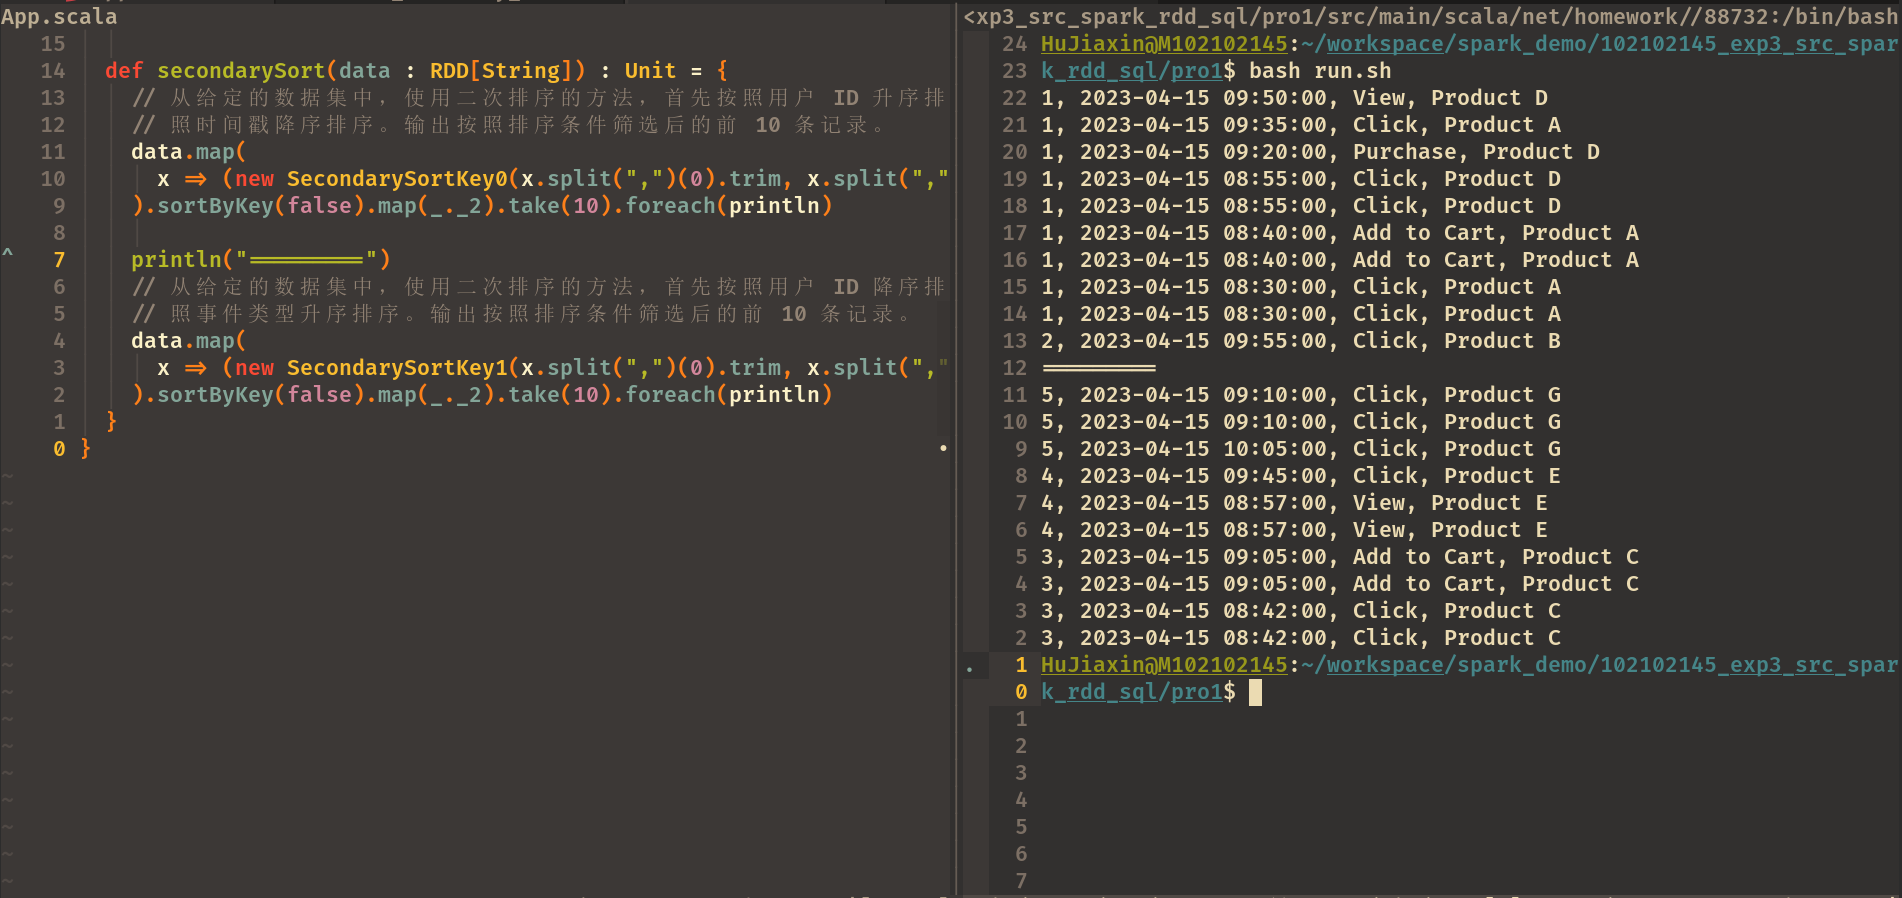
\includegraphics[width=0.95\textwidth]{./figures/1-1.png}
  \end{center}
  \caption{运行结果}
\end{figure}


\subsubsection{去重和统计}
\begin{itemize}
  \item 从给定的数据集中,找出重复的事件记录(完全相同的记录),并将它们去重。
    输出去重后的数据集。输出的数据格式:用户 ID 事件类型 事件内容
  \item 对去重后的数据集,统计每种事件类型的数量,并输出事件类型和对应的数量。
\end{itemize}

\begin{figure}[H]
  \begin{center}
    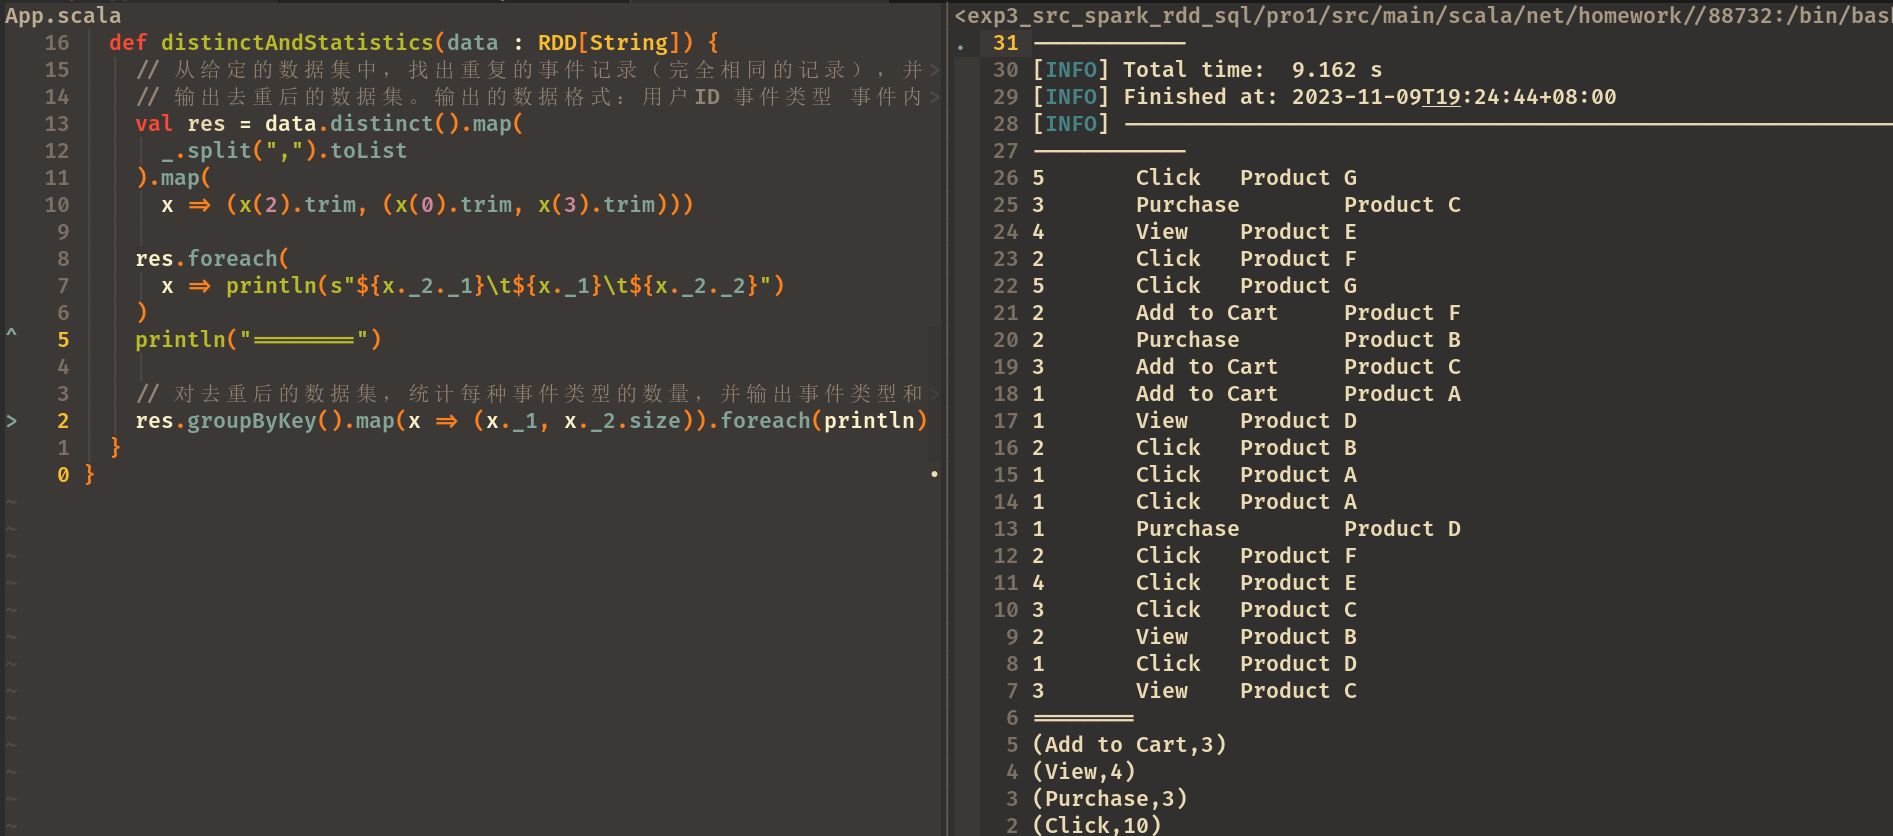
\includegraphics[width=0.95\textwidth]{./figures/1-2.png}
  \end{center}
  \caption{运行结果}
\end{figure}

\subsubsection{数据连接和格式化}

从用户信息数据集中读取用户 ID 和用户名称。将两个数据集根据用户 ID 进行连
接,得到一个新的数据集,其中包含用户信息和相关用户行为记录。

\begin{itemize}
  \item 对连接后的数据集进行进一步处理,将用户信息和活动详情合并成一个格式化的
    字符串,例如:"用户名称 - 事件类型 - 事件内容"。
  \item 输出格式化后的报告,包括每个用户的用户名称、事件类型和事件数量。
    输出格式为:用户名称--事件类型--事件数量
\end{itemize}

\begin{figure}[H]
  \begin{center}
    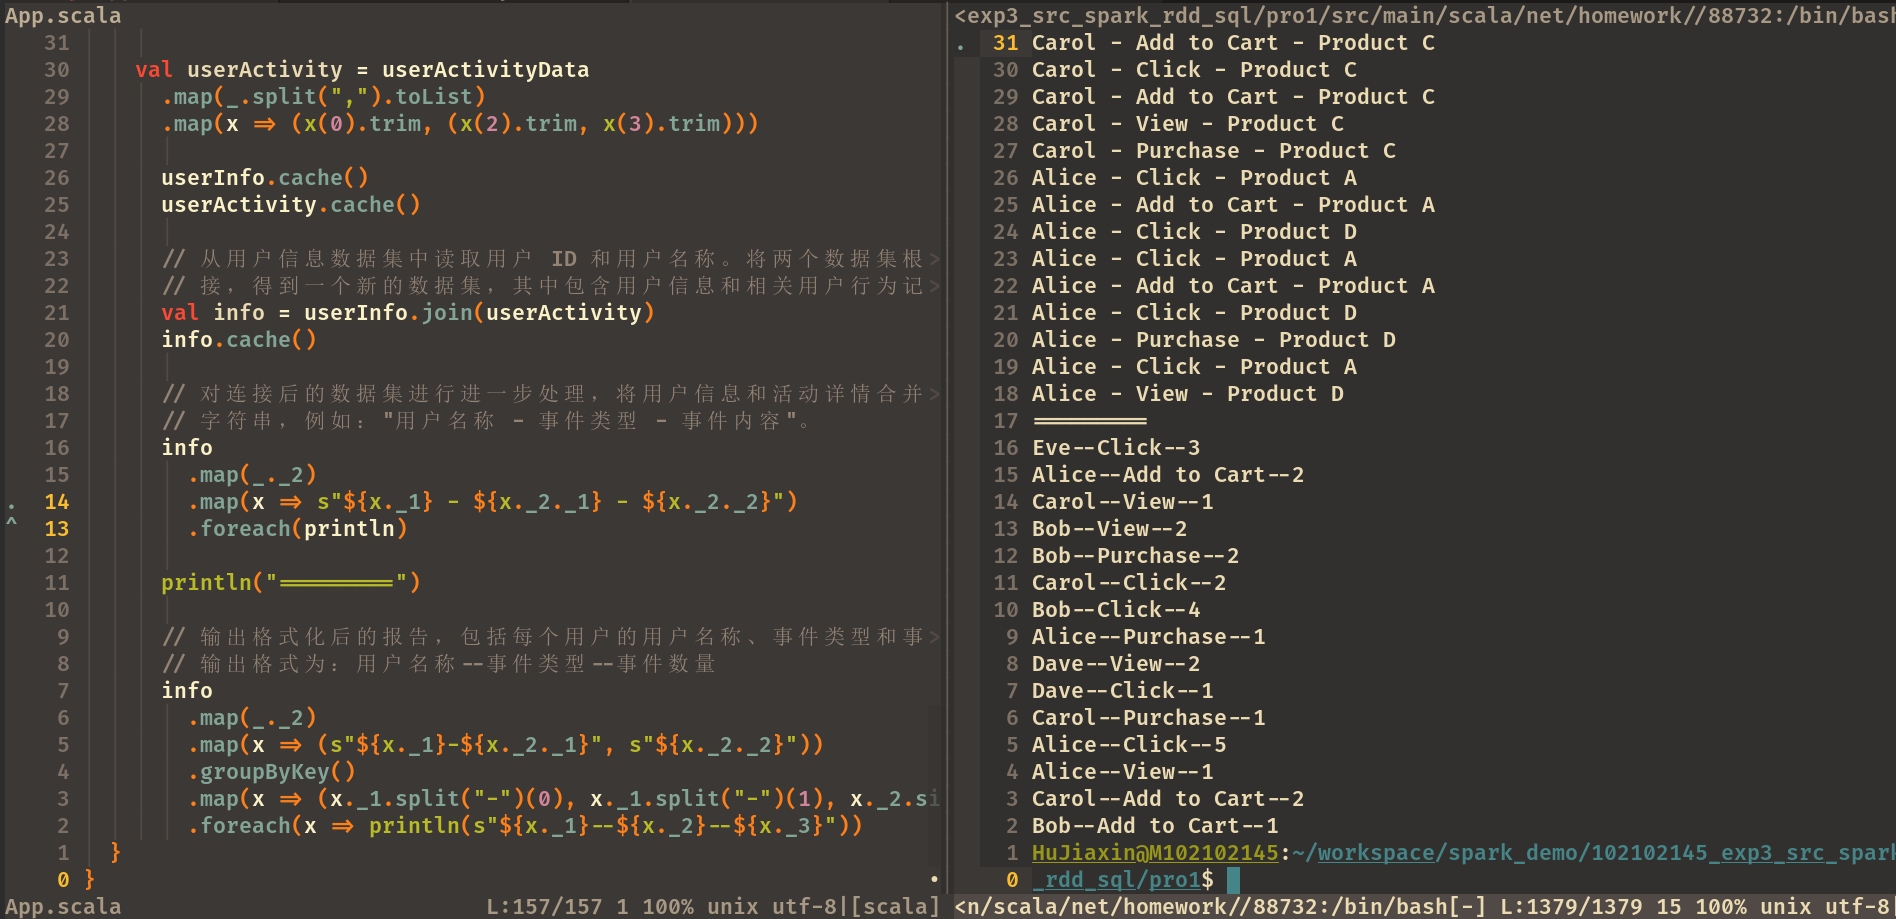
\includegraphics[width=0.95\textwidth]{./figures/1-3.png}
  \end{center}
  \caption{运行结果}
\end{figure}

\subsection{分析校运动会数据}

有一份运动会竞赛结果的数据集,其中包括比赛项目、班级、运动员、成绩和名次。
使用 Spark SQL 进行分析。

\subsubsection{计算所有比赛项目的平均成绩}
\begin{figure}[H]
  \begin{center}
    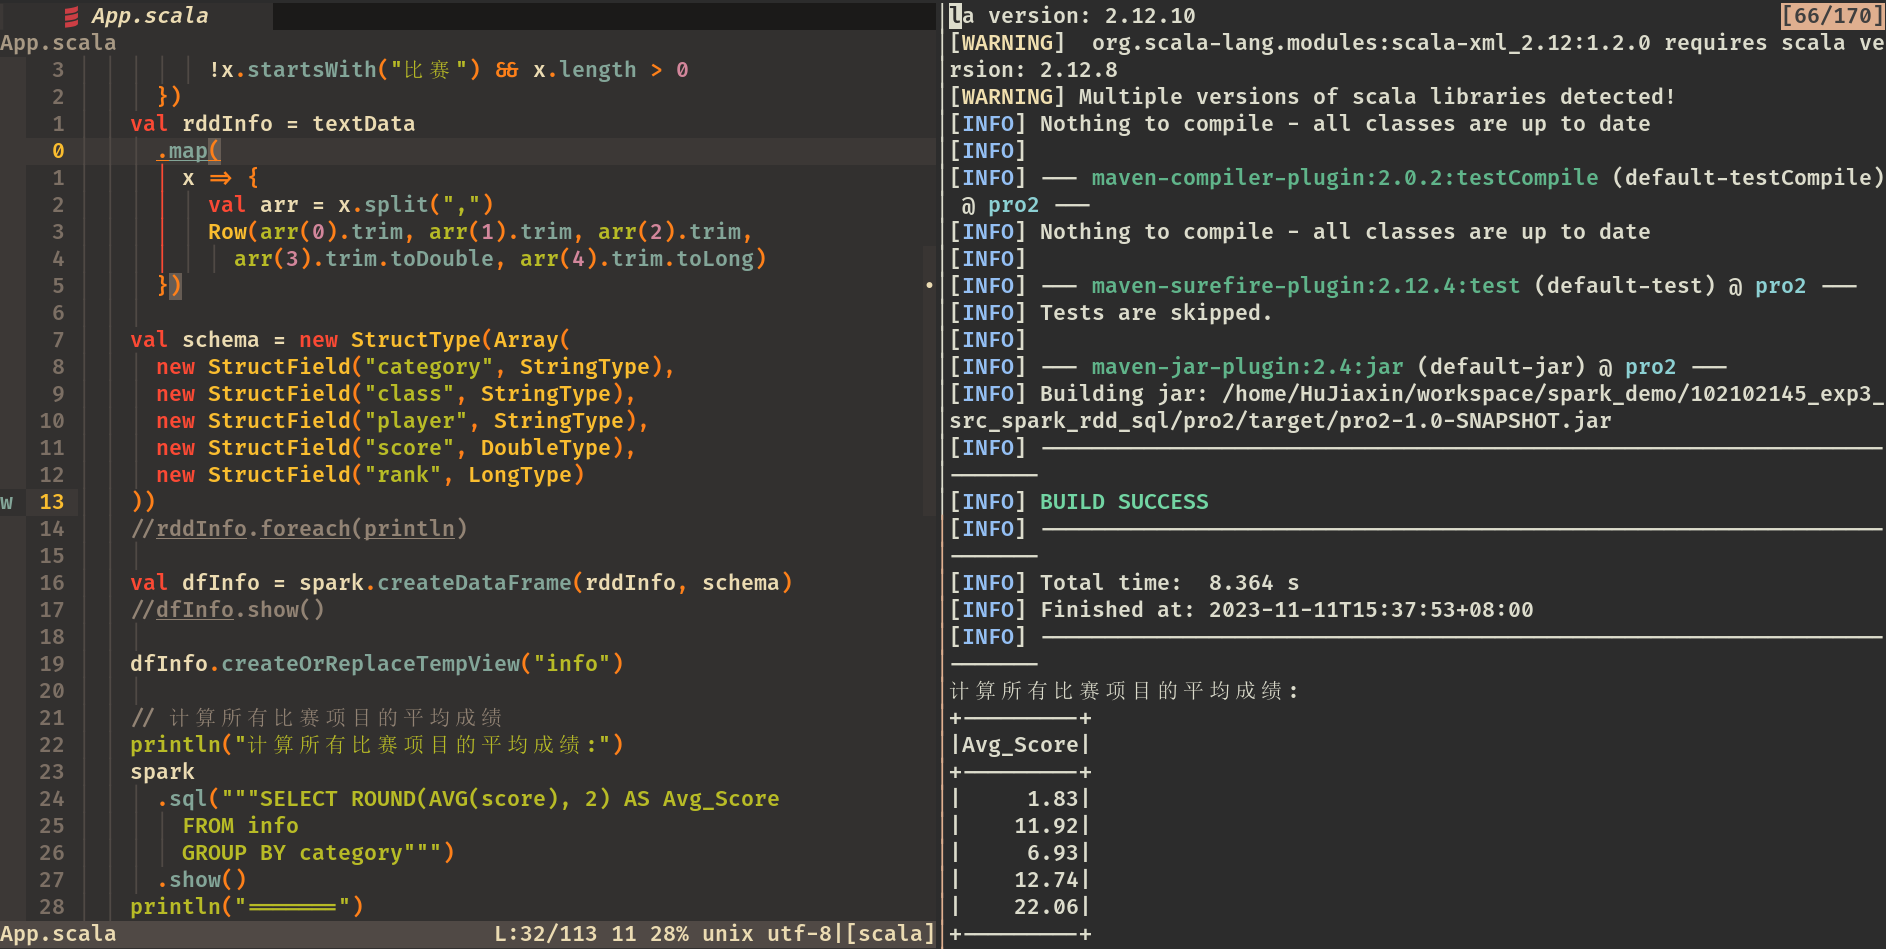
\includegraphics[width=0.95\textwidth]{./figures/2-1.png}
  \end{center}
  \caption{运行结果}
\end{figure}

\subsubsection{统计每个班级的名次总数}
\begin{itemize}
  \item 统计每个班级获得的第一名、第二名和第三名的次数。
  \item 列出获得第一名次数超过 2 次的班级。
\end{itemize}

\begin{figure}[H]
  \begin{center}
    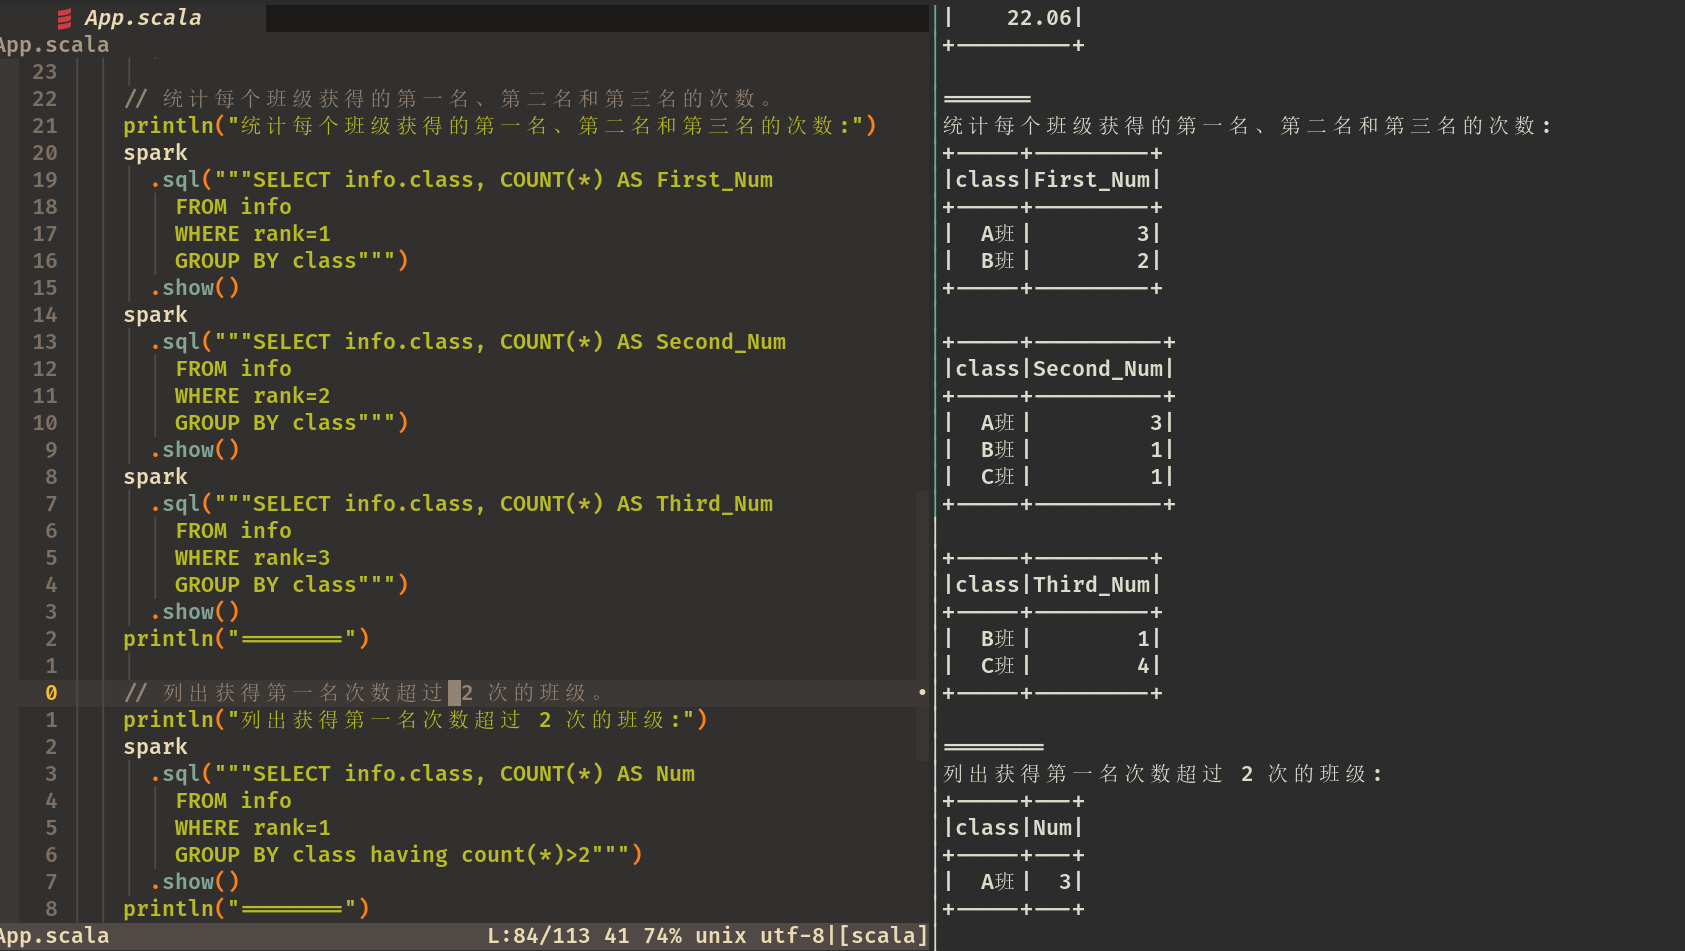
\includegraphics[width=0.95\textwidth]{./figures/2-2.png}
  \end{center}
  \caption{运行结果}
\end{figure}

\subsubsection{筛选并统计特定项目的成绩}
\begin{itemize}
  \item 筛选出所有田径项目(如 100 米短跑、200 米短跑)的比赛结果。
  \item 统计在这些田径项目中获得前三名的个人数量。
\end{itemize}

\begin{figure}[H]
  \begin{center}
    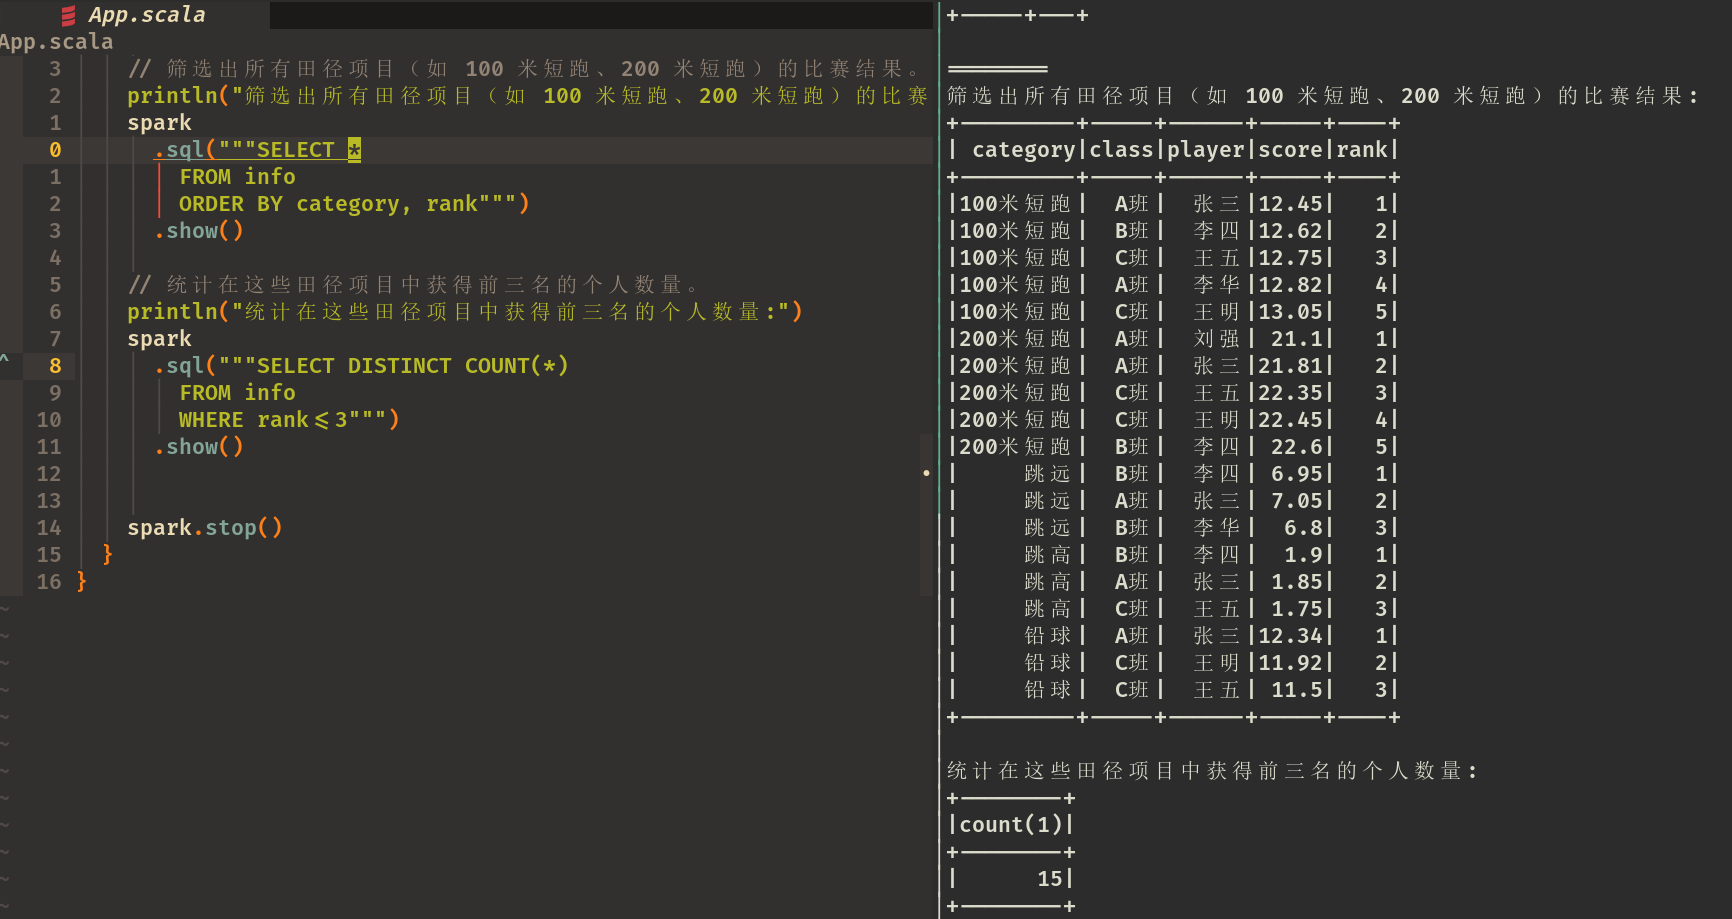
\includegraphics[width=0.95\textwidth]{./figures/2-3.png}
  \end{center}
  \caption{运行结果}
\end{figure}

\section{出现的问题及其解决方案}
没有问题.
\end{document}
